% Block structure of the Heisenberg Hamiltonian in Sz sectors, L = 6 (Session 2).
% Block dimensions binom(6, 3+m) = 1, 6, 15, 20, 15, 6, 1; total 2^6 = 64.
% Own drawing (Fable). Compile with: pdflatex sz_blocks.tex ; result moves to ../sz_blocks.pdf
\documentclass[11pt,tikz,border=3pt]{standalone}
\usepackage{amsmath,amssymb}
\usepackage{xcolor}
\definecolor{coursedark}{HTML}{1B2A4A}
\definecolor{courseaccent}{HTML}{7A2E8C}

\begin{document}
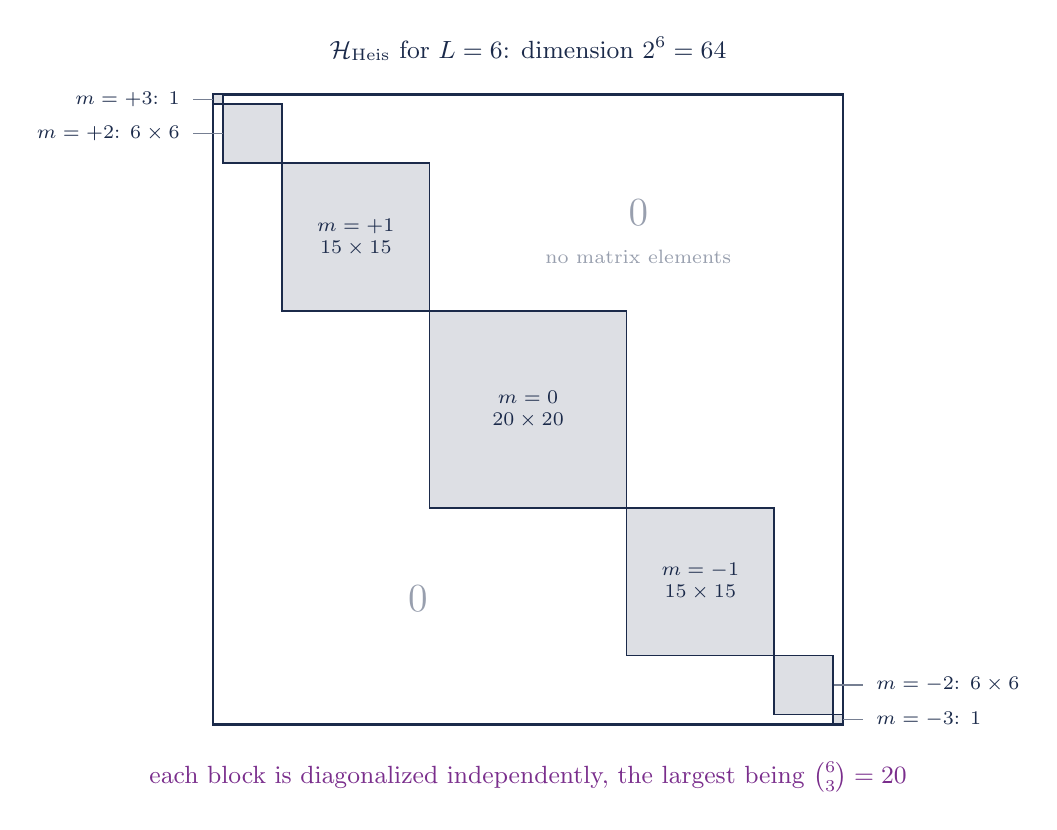
\begin{tikzpicture}[
    lbl/.style={font=\small, text=coursedark, align=center},
    idx/.style={font=\scriptsize, text=coursedark, align=center},
  ]
  \node[lbl, anchor=south] at (4,0.30)
    {$\mathcal{H}_{\mathrm{Heis}}$ for $L=6$: dimension $2^6=64$};
  \draw[coursedark, line width=1.0pt] (0,0) rectangle (8,-8);

  % diagonal blocks, 0.125 cm per basis state
  \foreach \xa/\xb in {0/0.125, 0.125/0.875, 0.875/2.75, 2.75/5.25,
                       5.25/7.125, 7.125/7.875, 7.875/8}{
    \fill[coursedark!15] (\xa,-\xa) rectangle (\xb,-\xb);
    \draw[coursedark, line width=0.6pt] (\xa,-\xa) rectangle (\xb,-\xb);
  }

  % labels inside the three big blocks
  \node[idx] at (1.8125,-1.8125) {$m={+}1$\\ $15\times15$};
  \node[idx] at (4,-4)           {$m=0$\\ $20\times20$};
  \node[idx] at (6.1875,-6.1875) {$m={-}1$\\ $15\times15$};

  % small blocks labeled outside with leaders
  \node[idx, anchor=east] at (-0.30,-0.0625) {$m={+}3$: $1$};
  \draw[coursedark!60, line width=0.5pt] (-0.25,-0.0625) -- (0.0,-0.0625);
  \node[idx, anchor=east] at (-0.30,-0.5) {$m={+}2$: $6\times6$};
  \draw[coursedark!60, line width=0.5pt] (-0.25,-0.5) -- (0.12,-0.5);
  \node[idx, anchor=west] at (8.30,-7.5) {$m={-}2$: $6\times6$};
  \draw[coursedark!60, line width=0.5pt] (8.25,-7.5) -- (7.88,-7.5);
  \node[idx, anchor=west] at (8.30,-7.9375) {$m={-}3$: $1$};
  \draw[coursedark!60, line width=0.5pt] (8.25,-7.9375) -- (8.0,-7.9375);

  % off-diagonal regions
  \node[text=coursedark!45] at (5.4,-1.5) {\Large $0$};
  \node[idx, text=coursedark!45, anchor=north] at (5.4,-1.85) {no matrix elements};
  \node[text=coursedark!45] at (2.6,-6.4) {\Large $0$};

  \node[lbl, text=courseaccent, anchor=north] at (4,-8.35)
    {each block is diagonalized independently, the largest being $\binom{6}{3}=20$};
\end{tikzpicture}
\end{document}
